% Created 2023-02-19 So 18:42
% Intended LaTeX compiler: pdflatex
\documentclass[11pt]{article}
\usepackage[utf8]{inputenc}
\usepackage[T1]{fontenc}
\usepackage{graphicx}
\usepackage{longtable}
\usepackage{wrapfig}
\usepackage{rotating}
\usepackage[normalem]{ulem}
\usepackage{amsmath}
\usepackage{amssymb}
\usepackage{capt-of}
\usepackage{hyperref}
\usepackage[a4paper,width=150mm,top=25mm,bottom=25mm]{geometry}
\author{Geeju Kwon, Jiawei Sun, Philip Wolper}
\date{\today}
\title{Simulation of wheat yield in the Cerrado region of Southern Brazil using the SIMPLE crop model}
\hypersetup{
 pdfauthor={Geeju Kwon, Jiawei Sun, Philip Wolper},
 pdftitle={Simulation of wheat yield in the Cerrado region of Southern Brazil using the SIMPLE crop model},
 pdfkeywords={},
 pdfsubject={},
 pdfcreator={Emacs 27.1 (Org mode 9.6)}, 
 pdflang={English}}
\begin{document}

\maketitle

\section{Introduction}
\label{sec:orgd61d6e2}
The Cerrado region of Brazil refers to the tropical savanna biomes that are widely distributed in the Eastern states of the country.In general, the climate of Cerrado region is characterized by the semi humid tropical regimes that are dominated by wet and cold seasons annually. Conventionally, Brazil’s wheat production is distributed in the Southern regions of Brazil, contributing up to 91 \% of national production in 2017. Although not considered a traditional region of cereal production, the Cerrado has become the target of agricultural expansion since the 1980s, due to its potential to grow wheat in the off-seasons from that of the Southern regions. It is worth noting that the Cerrado is a topic of interest due to its unprecedented agronomic background. For example, the seasonal variation of water usage and the blast disease caused by the fungus \emph{Pyricularia oryzae} are identified as significant threats to long-term productivity and yield stability. The incentive of agricultural expansion into the Cerrado is considered to be a lucrative development in the region, partitioning approximately 44\% of its total area to farmland. However, Brazil’s agroeconomic reliance on such expansions may highlight the increasing vulnerability to anthropogenic climate change, which could destabilize crop production to meet the domestic food demand. Recognizing the impacts of the progressing agricultural expansion, the employment of crop system simulations could offer a sustain growth model for shareholders, legislators, and farmers. Moreover, the development of simulated crop models could illuminate the crucial system components and its interrelationships involved in crop production, overcoming agronomic challenges.\\

\begin{figure}[htbp]
\centering
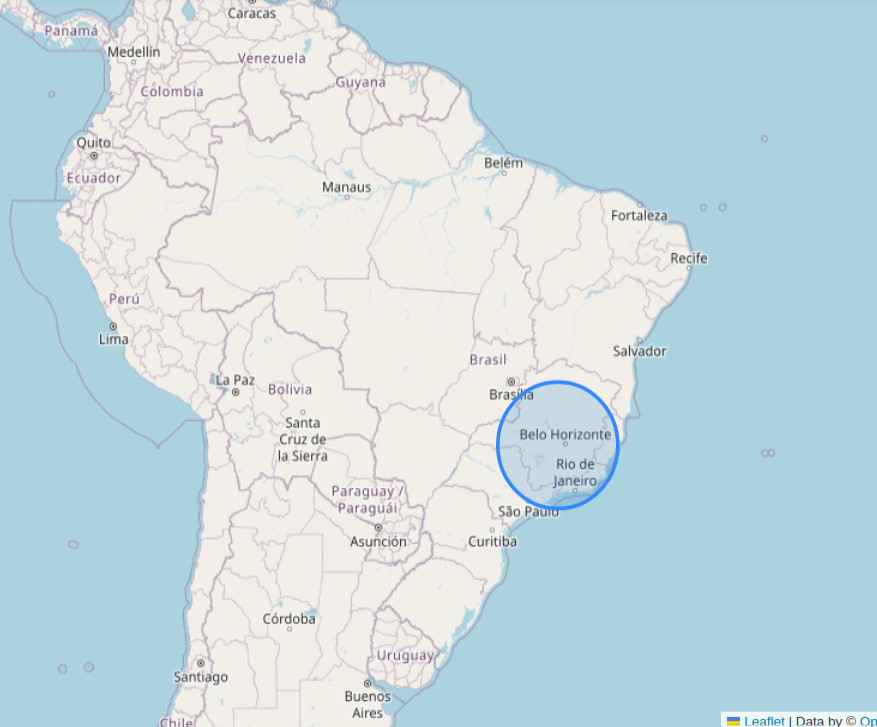
\includegraphics[width=0.5\textwidth]{./figures/Brazil with cerrado.png}
\caption{Relative location of the Cerrado in Brazil. The circle encloses the area .}
\end{figure}

\section{Objectives and Aims}
\label{sec:org2171bc5}
This study aims to utilize the SIMPLE crop model developed by Zhao et al. to simulate crop production in the Cerrado region at various locations and temporal scales. Additionally, this study intends to explore the model’s statistical fit for wheat yield simulations in relation to the observed experimental data. Simultaneously, the model’s response to a changing climate will be assessed under the conditions presented in RCP 8.5 climate change model. Although several models have been extensively developed for wheat, the SIMPLE crop model is selected for the study due to its relatively simple yet dynamic nature. Notably, the integration of widely understood processes with few parameters and data requirements that exclude crop-specific processes, is considered the appeal of utilizing the SIMPLE model.

\section{Experimental Data}
\label{sec:orgd93afc6}
Experimentally determined wheat yield was collected for 13 field trials from five experimental sites located in the Cerrado (Rio Paranaíba, Viçosa, São Gotardo, Sete Lagoas, and Itutinga) (\textbf{Table and Figure}, who to site). The field trials were conducted between 2018 and 2021 and were conducted with the wheat cultivar BRS264, which is the most widely grown and consumed culitvar in the Cerrado since the last 10 years, due to its tolerance to heat, pathogens, water lodging and toxic metal elements commonly found in Cerrado soils. While the sowing date varies between locations and experiments, on average the wheat was sown on the 20th of May and harvested on the 19th of September. This timeline coincides with the recommendation for this cultivar (\textbf{cite by who}). Because we did not have access to detailed soil data for each location, soil parameters were approximated from the average content of clay, sand and silt in the Cerrado (\textbf{site soil content}). Using the Unified Soil Classification System Pyramid, this yielded a soil with sandy loamy characteristics. The 13 field trials included both irrigated and non-irrigated experiments, but no further data on the amount of irrigation was supplied. While for most field trials various environmental conditions are controlled such as nutrient saturation and disease control, it is very important to note that wheat grwon under nonirrigated conditions in the location São Gotardo was artificially inoculated with the fungal pathogen \emph{Magnaporthae oryzae} pv. \emph{Triticum}, which causes wheat blast disease.

\begin{figure}[htbp]
\centering
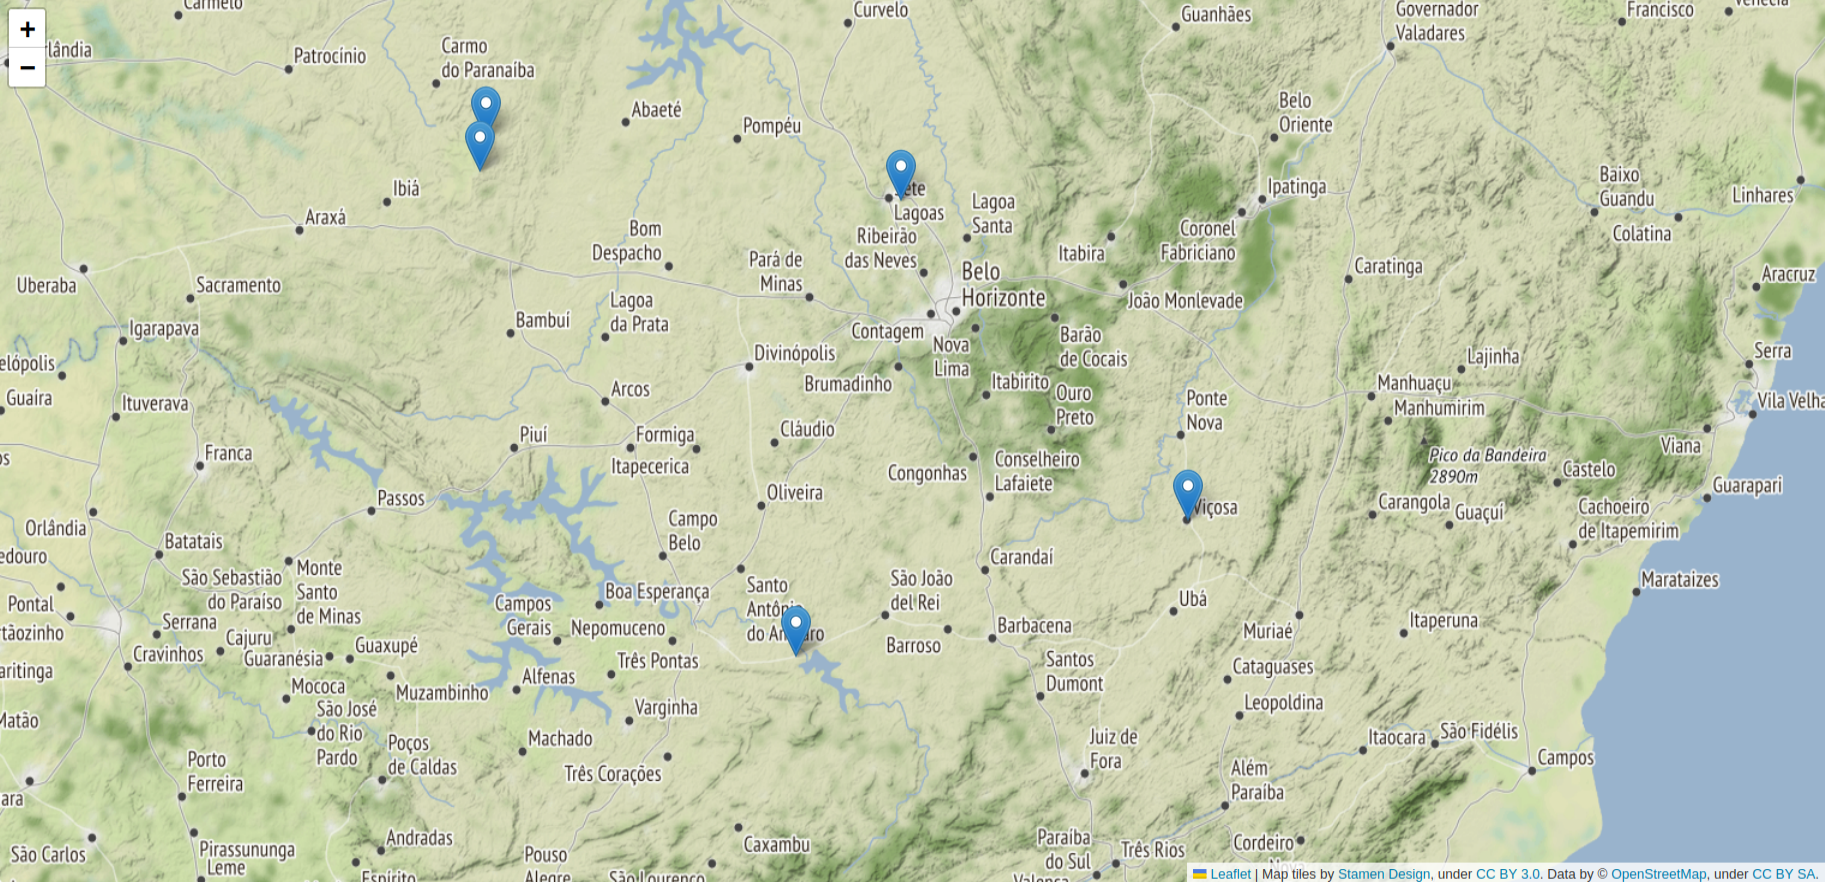
\includegraphics[width=0.9\textwidth]{./figures/Brazil.png}
\caption{Location of the field trials in the Cerrado in Brazil, which were simulated in this study.}
\end{figure}


\section{SIMPLE model}
\label{sec:orgb015e4b}

\section{Results}
\label{sec:orga75bd59}
\subsection{Simulated experiments}
\label{sec:orgadb2cc5}
In order to assess the capabilities of the SIMPLE model to model wheat growth in the Cerrado region, we simulated yield for 13 field trials in 5 different locations. Irrigated location where simulated with no water stress, implying a perfect watering routine. Nonirrigated crops had water stress turned on and relied only on rainfalls, supplied in the weather data. Since no nutrients are simulated in the SIMPLE model, we assume perfect nutrient saturation of the crops, a state not uncommon for field trials. The atmospheric CO2 concentration was set to 415 ppm, reflecting the current value as of 2020. Soil parameters were estimated from the content of Silt, Clay and Sand found in typical Cerrado soils (\textbf{cite soils})

The species and cultivar parameters required by the SIMPLE mode were derived from literature or estimated based on similar species. (\textbf{cite zhao et al.}) Further calibration was done by adjusting cultivar parameters (Tsum, I50A, I50B and HI) within reasonable levels.

(insert table here.)

The results of the simulation across experiments are shown in (Figure calibration). The model has an accuracy of:

\begin{figure}[htbp]
\centering
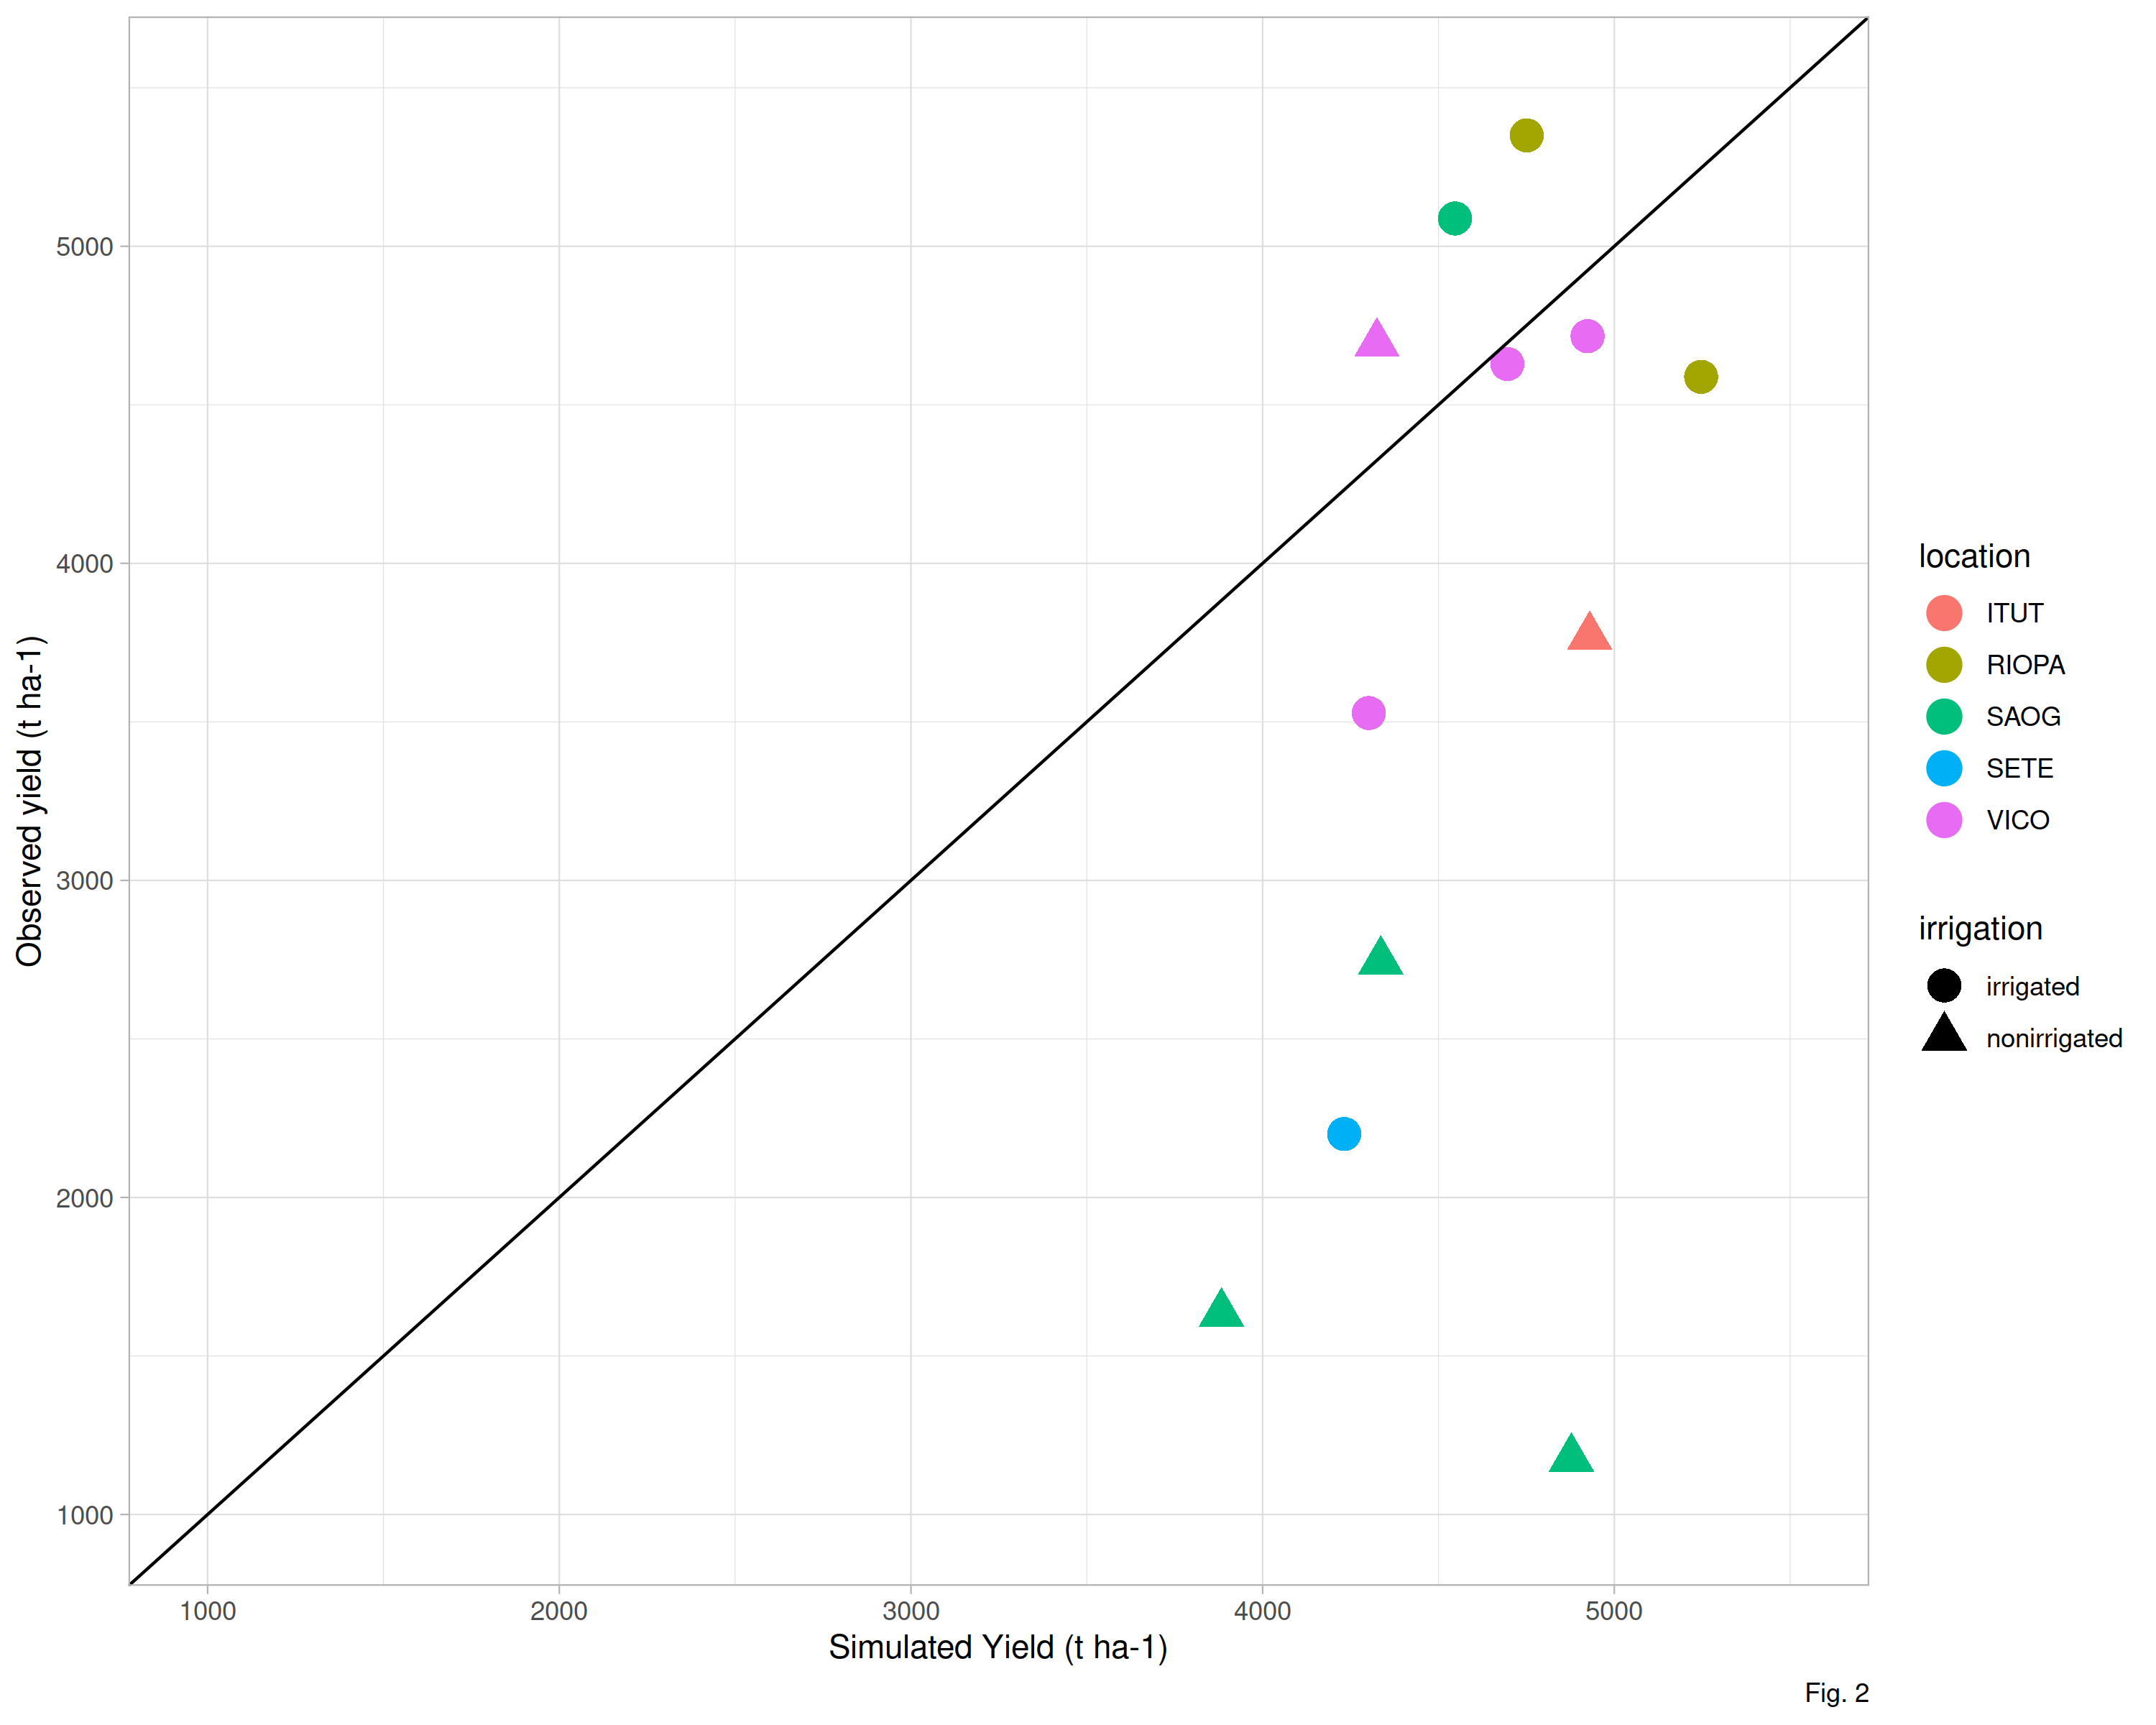
\includegraphics[width=.9\linewidth]{../results/experimental-data/2023-02-18_Obs_Sim_all_415.png}
\caption{Simulated vs. Observed yield for 13 field trial locations in the Cerrado, Brazil.}
\end{figure}

These results indicate that in many cases there is significant deviation between the simulated and observed yield. While several experiments are simulated with decent accuracy, a general trend of the simulation to overestimating the observed yield can be observed. Due to the simple nature of the model this is to be expected, since in reality there are many more yield-limiting factors, such as nutrients, that the SIMPLE model does not account for.
We also observe that the accuracy of predicting yield varies between locations, as can  be expected between differing environments. It can be seen, that experiments conducted in Vicosa, MG have the best simulated results of all 5 locations. On the other hand, specifically the nonirrigated field trials in Sao Gotardo, which also have been inoculated with a fungal pathogen, show a bad fit between simulated and observed yield, by grossly overestimating the yield in the simulation. This discrepancy is likely caused by the fungal pathogen having a negative effect on the yield, which is not accounted for by the model.

\begin{table}[htbp]
\caption{\label{stats}Model statistics\\
}
\centering
\begin{tabular}{|c|c|c|c|c|}
\hline
 & r\textsubscript{squared} & mae & rmse & md\\
\hline
All & 0.226 & 1131.89 & 1499.29 & 0.435\\
healthy & 0.254 & 717.22 & 890.4 & 0.349\\
Vicosa & 0.336 & 354.35 & 442.34 & 0.479\\
\hline
\end{tabular}
\end{table}

Summary statistics decribing the accuracy are done for all experiments, as well as subgroups of the data. These can be seen in Table \ref{stats} and include all the experiments (All), excluding the nonirrigated trials in Sao Gotardo, where the plants where infected with the blast fungus (healthy) and statistics of only the trials in Vicosa (Vicosa), where the model performed the most accurately.

\begin{center}
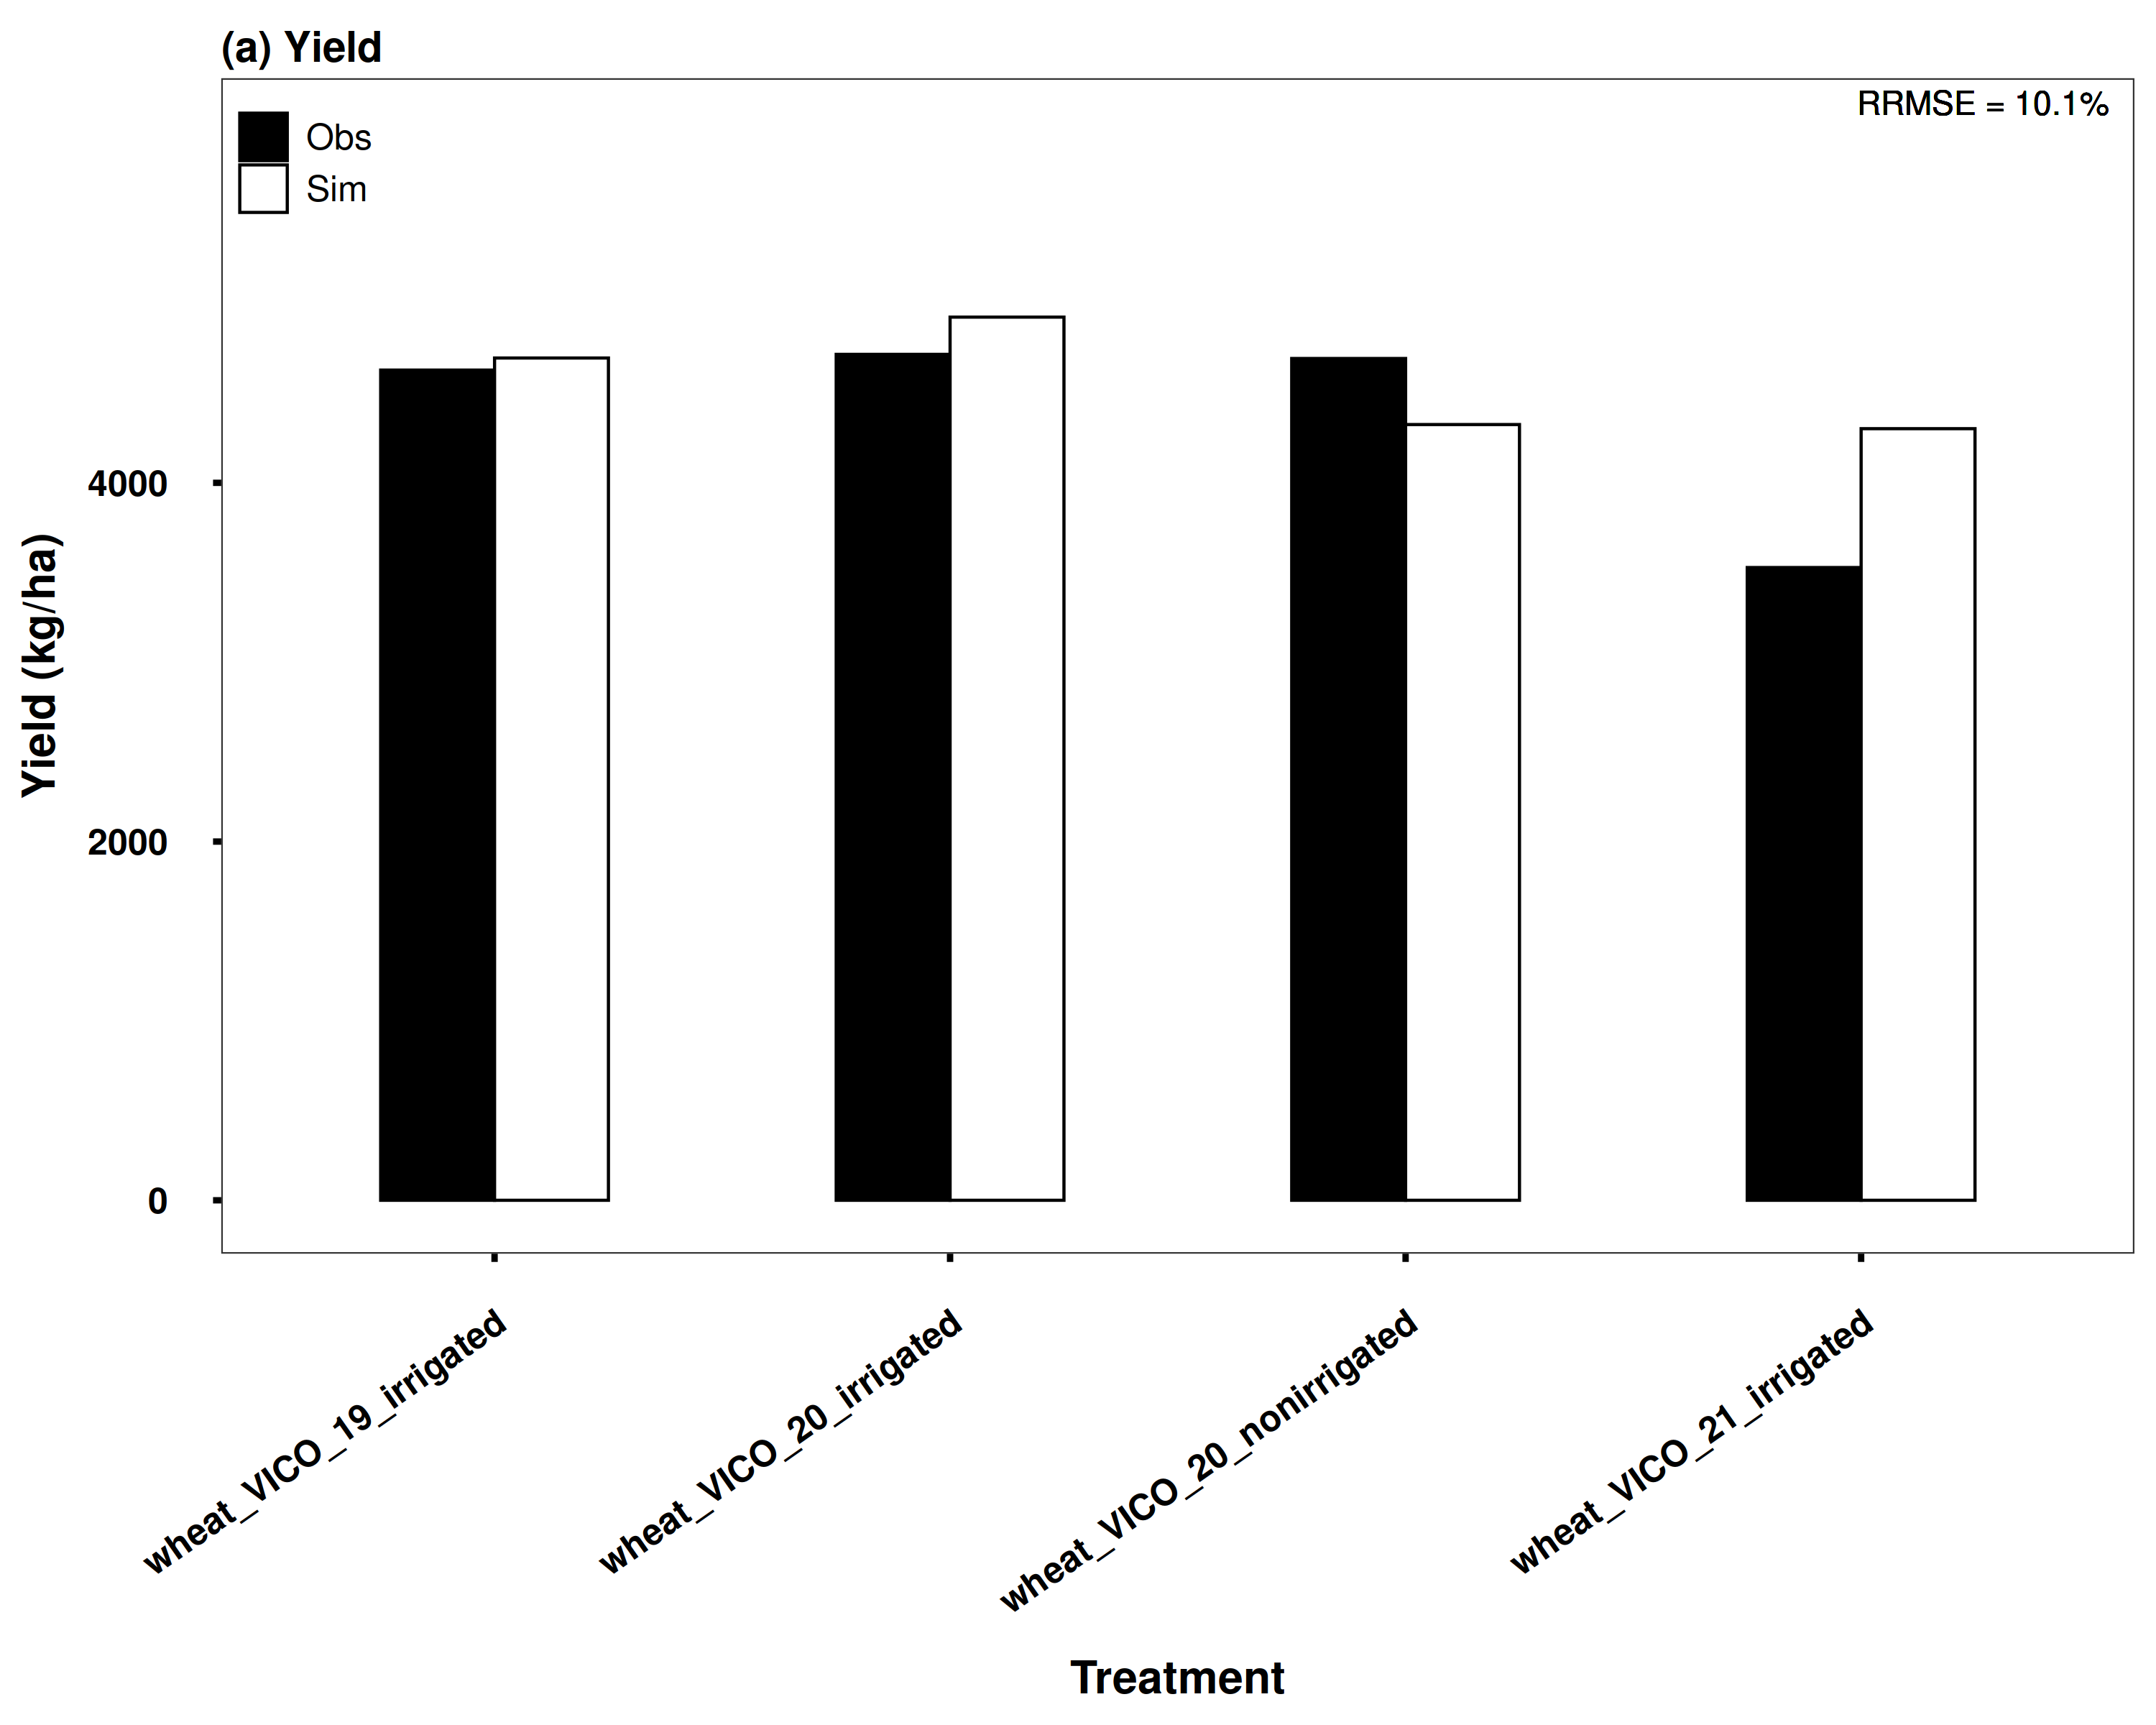
\includegraphics[width=.9\linewidth]{../results/experimental-data/2023-02-18_Vico_only.png}
\end{center}


\subsection{Climate change prediction}
\label{sec:org6e7b0cd}
As the amount of greenhouse gases (GHG) released by humans and their societies predicted to further increase during the second half of the century it, it's impact on agriculture is important for maintaining food security during a changing climate. As it is the most common GHG emitted by humans and contributes greatly to global warming the levels of CO\textsubscript{2} in the atmosphere have been subject to much predictive modeling. According to the latest IPCC (\textbf{cite}) report, by the end of the 21st Century the concentration of CO\textsubscript{2} in the atmosphere is predicteed to increase to levels anywhere between 400 ppm to 1100 ppm. While the lower limit of this prediction depends on the most favorable scietal drivers involving drastic reductions in emission very rapidly, the upper limits assumes the most detrimental course of society, involving little to no climate action. While both of these szenarios are considered unlikely, mean CO\textsubscript{2}-concentration in the atmosphere is still likely to increase by up to 50\% under realistic szenarios.

In order to simulate the effect of increasing atmospheric CO\textsubscript{2} concentrations on wheat yield in the brazilian Cerrado, we will assume a linear increase of CO\textsubscript{2} and reaches 795 ppm by the year 2100. Because our simulation starts in the year 2030, we have choose an appropriate concentration of 450 ppm as a starting value, and assume an increase by 5 ppm.

\begin{figure}[htbp]
\centering
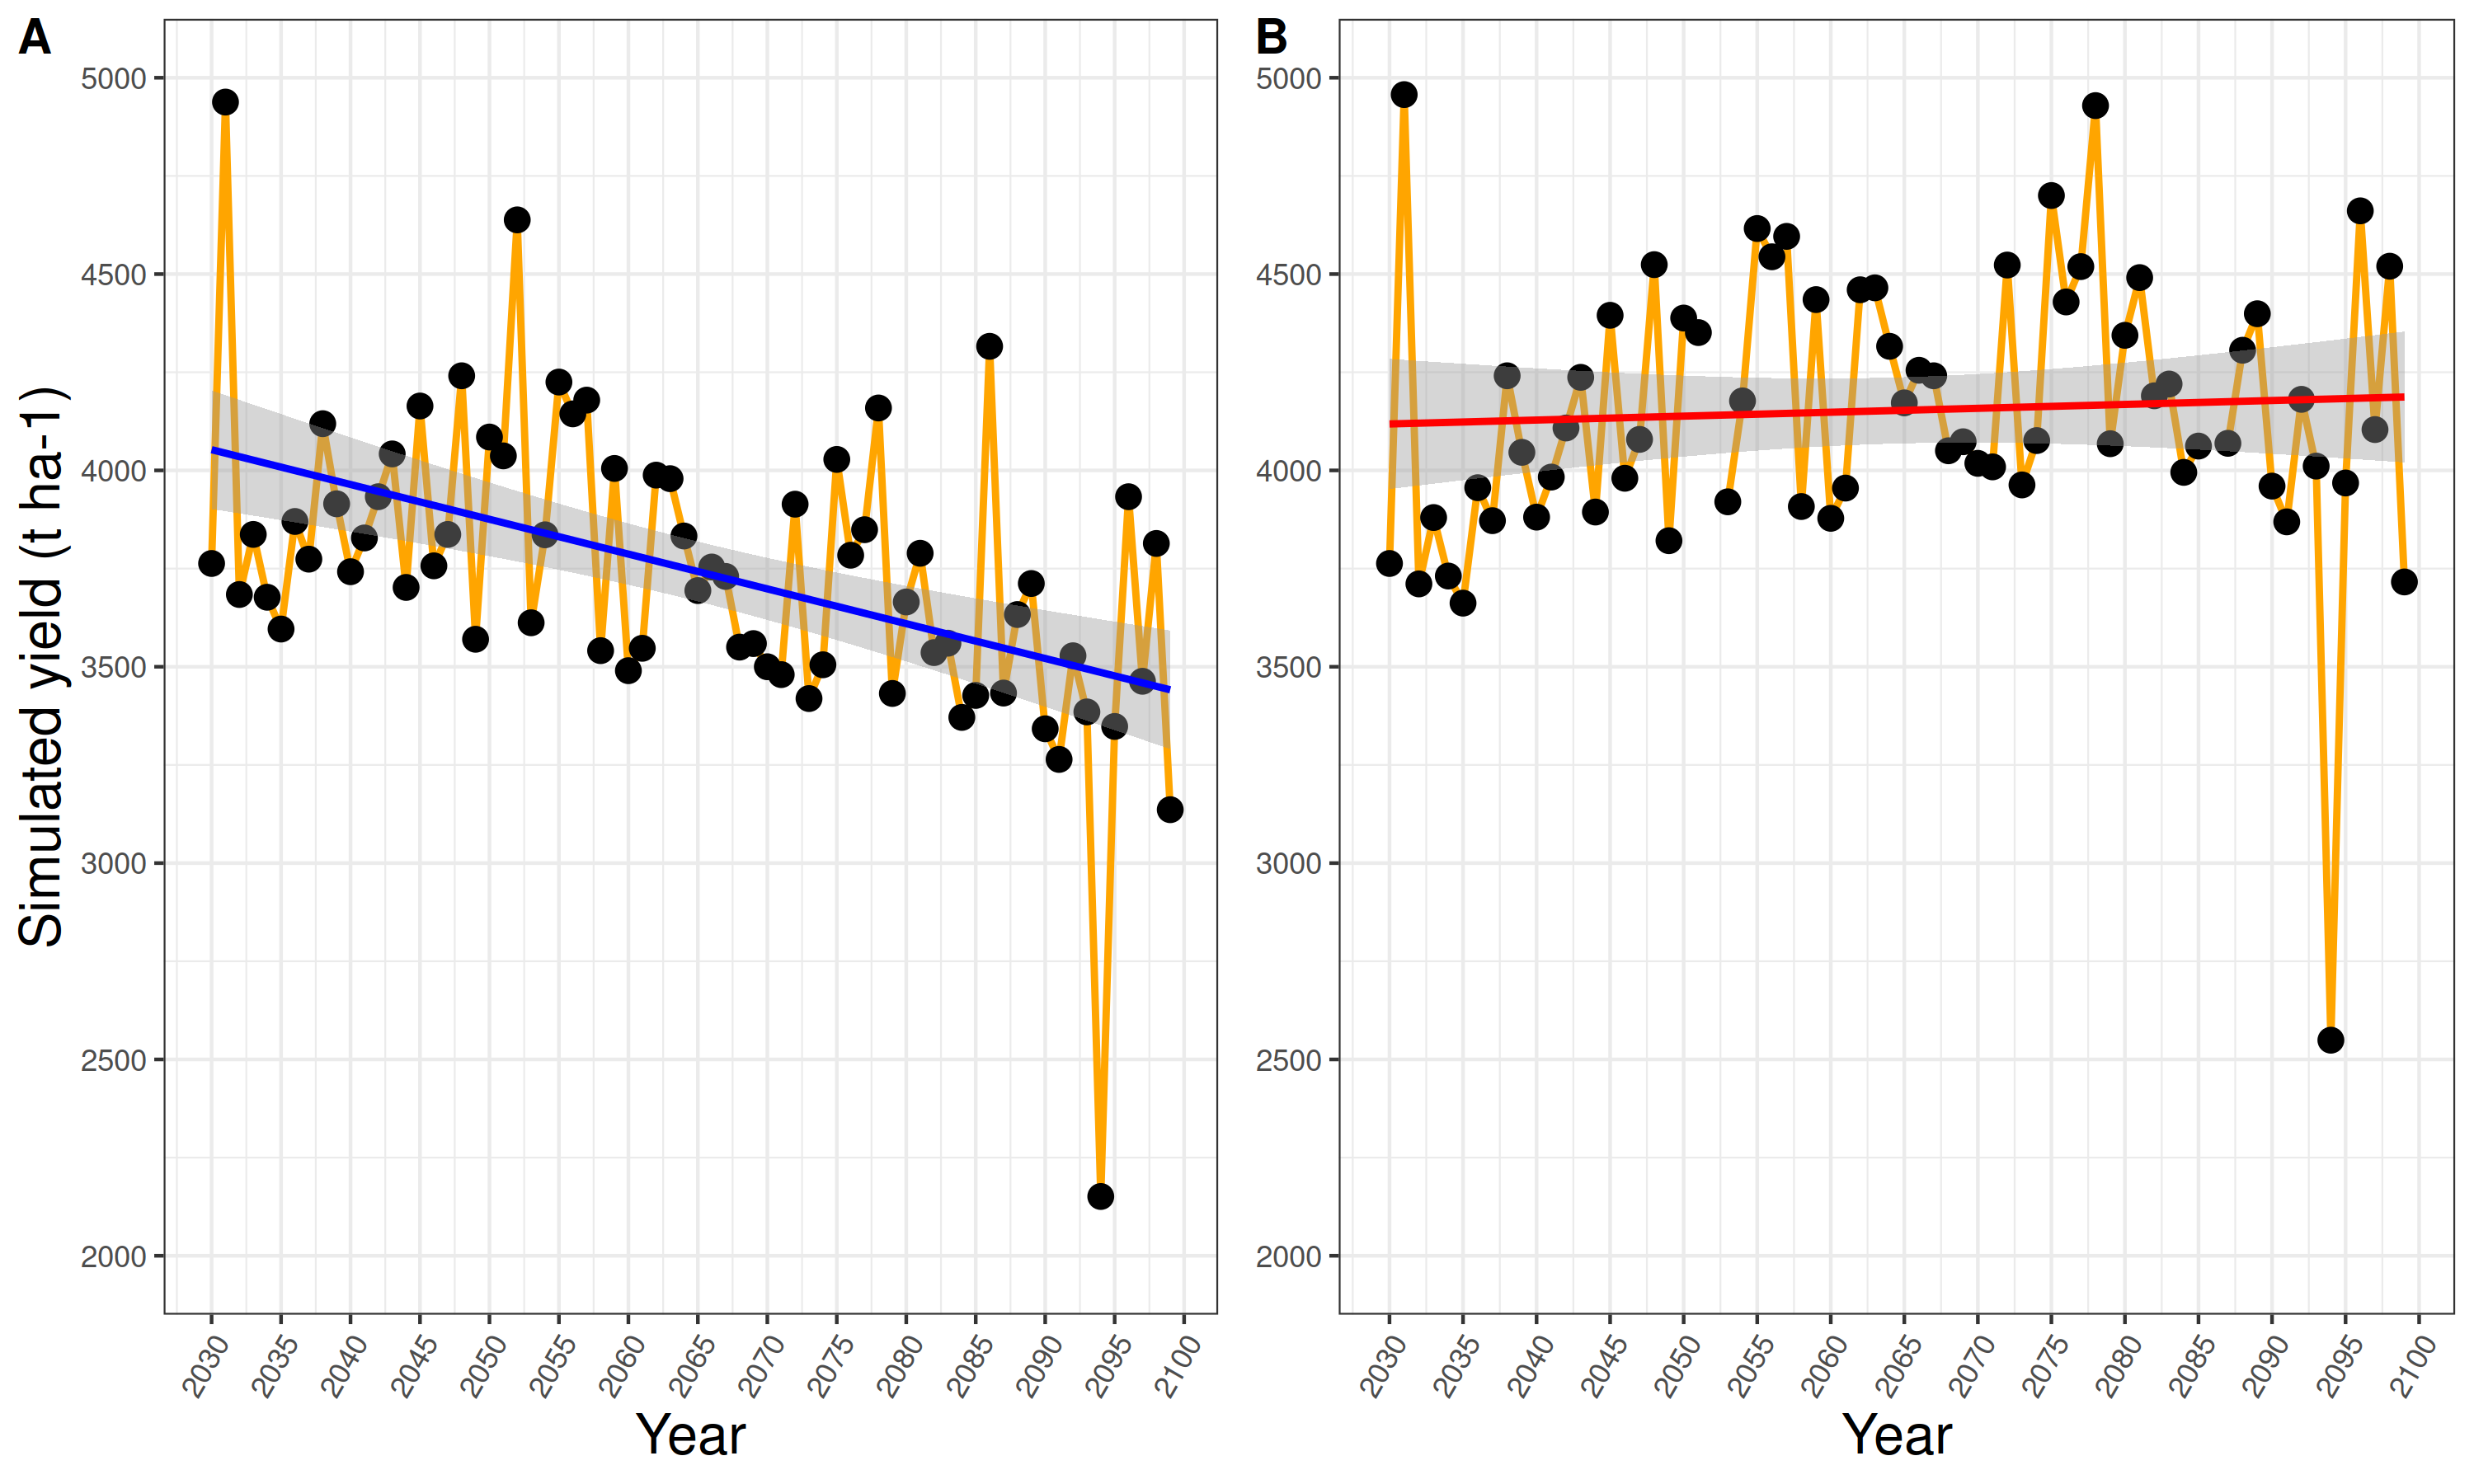
\includegraphics[width=.9\linewidth]{../results/cc-model/2023-02-19_yield_prediction_cc_model_CO2.png}
\caption{Climate change model}
\end{figure}

\section{Discussion}
\label{sec:orga018c27}
\end{document}
